% questions.tex —— 2013 年·春季上海卷 · 题目内容片段（无答案）
% 由 tools/generate_projects.py 依来源总账自 2013/2013_数学真题_春季上海_试题.md 生成，勿手改（改源 MD 后重跑）


\begin{gktip}
\textbf{来源说明}：本题面依据固定源 PDF 的第 1—7 页逐题转录，原卷印刷页码为 1/7—7/7；第 8—11 页为官方参考答案与详细解答，答案证据等级 A。第 8 题原卷印面作“$b=8$”，与同句所问“则 $b=$”及参考答案 $7$ 矛盾，当为“$c=8$”之误；本稿按 $a=5$、$c=8$、$B=60^\circ$ 转录，并在解析中说明。

\textbf{答案归属}：源内附官方答案与详细解答；本稿答案与解析以第 8—11 页为底稿整理，关键中间量均已复算。

\textbf{图形说明}：第 9 题正方体、第 16 题四联图象、第 25 题正三棱柱、第 26 题直角三角形与内接矩形、第 30 题坐标系与点列，均由项目内 TikZ 矢量重绘。
\end{gktip}

\gkpart{一、填空题}

\begin{question}
\gkti{1}函数 $y=\log_2(x+2)$ 的定义域是\gkblank{}。

\end{question}
\begin{question}
\gkti{2}方程 $2^x=8$ 的解是\gkblank{}。

\end{question}
\begin{question}
\gkti{3}抛物线 $y^2=8x$ 的准线方程是\gkblank{}。

\end{question}
\begin{question}
\gkti{4}函数 $y=2\sin x$ 的最小正周期是\gkblank{}。

\end{question}
\begin{question}
\gkti{5}已知向量 $\boldsymbol a=(1,k)$，$\boldsymbol b=(9,k-6)$。若 $\boldsymbol a\parallel\boldsymbol b$，则实数 $k=$\gkblank{}。

\end{question}
\begin{question}
\gkti{6}函数 $y=4\sin x+3\cos x$ 的最大值是\gkblank{}。

\end{question}
\begin{question}
\gkti{7}复数 $2+3\mathrm i$（$\mathrm i$ 是虚数单位）的模是\gkblank{}。

\end{question}
\begin{question}
\gkti{8}在 $\triangle ABC$ 中，角 $A$、$B$、$C$ 所对边长分别为 $a$、$b$、$c$，若 $a=5$，$c=8$，$B=60^\circ$，则 $b=$\gkblank{}。

\Needspace{0.4\textheight}
\end{question}
\begin{question}
\gkti{9}在如图所示的正方体 $ABCD-A_1B_1C_1D_1$ 中，异面直线 $A_1B$ 与 $B_1C$ 所成角的大小为\gkblank{}。
\nopagebreak[4]
\begin{center}% 2013 年春季上海卷第 9 题：正方体 ABCD-A1B1C1D1
% 突出异面直线 A1B 与 B1C；图中透视比例不代表题设尺寸。
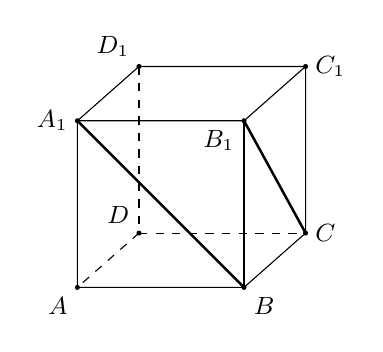
\begin{tikzpicture}[>=stealth, scale=0.92, font=\small]
  \coordinate (A)  at (0,0);
  \coordinate (B)  at (2.30,0);
  \coordinate (C)  at (3.15,0.75);
  \coordinate (D)  at (0.85,0.75);
  \coordinate (A1) at (0,2.30);
  \coordinate (B1) at (2.30,2.30);
  \coordinate (C1) at (3.15,3.05);
  \coordinate (D1) at (0.85,3.05);
  % 可见棱
  \draw (A) -- (B) -- (C) -- (C1) -- (B1) -- (A1) -- cycle;
  \draw (A1) -- (D1) -- (C1);
  \draw (B) -- (B1);
  % 不可见棱
  \draw[dashed] (D1) -- (D);
  \draw[dashed] (D) -- (C);
  \draw[dashed] (D) -- (A);
  % 异面直线 A1B 与 B1C
  \draw[line width=0.9pt] (A1) -- (B);
  \draw[line width=0.9pt] (B1) -- (C);
  % 顶点
  \fill (A) circle (1pt) node[below left] {$A$};
  \fill (B) circle (1pt) node[below right] {$B$};
  \fill (C) circle (1pt) node[right] {$C$};
  \fill (D) circle (1pt) node[above left] {$D$};
  \fill (A1) circle (1pt) node[left] {$A_1$};
  \fill (B1) circle (1pt) node[below left] {$B_1$};
  \fill (C1) circle (1pt) node[right] {$C_1$};
  \fill (D1) circle (1pt) node[above left] {$D_1$};
\end{tikzpicture}
\end{center}
\nopagebreak[4]
\end{question}
\begin{question}
\gkti{10}从 $4$ 名男同学和 $6$ 名女同学中随机选取 $3$ 人参加某社团活动，选出的 $3$ 人中男女同学都有的概率为\gkblank{}（结果用数值表示）。

\end{question}
\begin{question}
\gkti{11}若等差数列的前 $6$ 项和为 $23$，前 $9$ 项和为 $57$，则数列的前 $n$ 项和 $S_n=$\gkblank{}。

\end{question}
\begin{question}
\gkti{12}$36$ 的所有正约数之和可按如下方法得到：

\Needspace{5\baselineskip}
因为 $36=2^2\times3^2$，所以 $36$ 的所有正约数之和为

\nopagebreak[4]
\[(1+3+3^2)+(2+2\times3+2\times3^2)+(2^2+2^2\times3+2^2\times3^2)=(1+2+2^2)(1+3+3^2)=91.\]

参照上述方法，可求得 $2000$ 的所有正约数之和为\gkblank{}。

\end{question}
\gkpart{二、选择题}

\begin{question}
\gkti{13}展开式为 $ad-bc$ 的行列式是\mbox{（　　）}

（A）$\begin{vmatrix}a&b\\d&c\end{vmatrix}$；（B）$\begin{vmatrix}a&c\\b&d\end{vmatrix}$；（C）$\begin{vmatrix}a&d\\b&c\end{vmatrix}$；（D）$\begin{vmatrix}b&a\\d&c\end{vmatrix}$。

\end{question}
\begin{question}
\gkti{14}设 $f^{-1}(x)$ 为函数 $f(x)=\sqrt x$ 的反函数，下列结论正确的是\mbox{（　　）}

（A）$f^{-1}(2)=2$；（B）$f^{-1}(2)=4$；（C）$f^{-1}(4)=2$；（D）$f^{-1}(4)=4$。

\end{question}
\begin{question}
\gkti{15}直线 $2x-3y+1=0$ 的一个方向向量是\mbox{（　　）}

（A）$(2,-3)$；（B）$(2,3)$；（C）$(-3,2)$；（D）$(3,2)$。

\Needspace{0.4\textheight}
\end{question}
\begin{question}
\gkti{16}函数 $f(x)=x^{-\frac12}$ 的大致图像是\mbox{（　　）}
\nopagebreak[4]
\begin{center}% 2013 年春季上海卷第 16 题：f(x)=x^{-1/2} 的候选图像
% 四个小坐标系按原卷自左至右排列，依次标 (A)(B)(C)(D)。
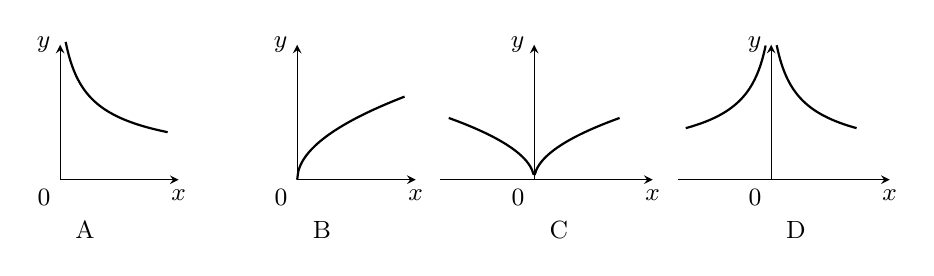
\begin{tikzpicture}[>=stealth, scale=0.70, font=\small]
  % (A) 定义域 x>0，单调递减
  \begin{scope}
    \draw[->] (0,0) -- (2.15,0) node[below] {$x$};
    \draw[->] (0,0) -- (0,2.45) node[left] {$y$};
    \node[below left] at (0,0) {$0$};
    \draw[thick, domain=0.10:1.95, samples=90, smooth]
      plot (\x,{1.25/sqrt(\x+0.15)});
    \node at (0.45,-0.92) {A};
  \end{scope}
  % (B) 过原点，单调递增
  \begin{scope}[xshift=4.30cm]
    \draw[->] (0,0) -- (2.15,0) node[below] {$x$};
    \draw[->] (0,0) -- (0,2.45) node[left] {$y$};
    \node[below left] at (0,0) {$0$};
    \draw[thick, domain=0:1.95, samples=90, smooth]
      plot (\x,{1.08*sqrt(\x)});
    \node at (0.45,-0.92) {B};
  \end{scope}
  % (C) 关于 y 轴对称，原点处取最小值
  \begin{scope}[xshift=8.60cm]
    \draw[->] (-1.70,0) -- (2.15,0) node[below] {$x$};
    \draw[->] (0,0) -- (0,2.45) node[left] {$y$};
    \node[below left] at (0,0) {$0$};
    \draw[thick, domain=-1.55:1.55, samples=120, smooth]
      plot (\x,{0.90*sqrt(abs(\x))});
    \node at (0.45,-0.92) {C};
  \end{scope}
  % (D) 关于 y 轴对称，两侧单调递减
  \begin{scope}[xshift=12.90cm]
    \draw[->] (-1.70,0) -- (2.15,0) node[below] {$x$};
    \draw[->] (0,0) -- (0,2.45) node[left] {$y$};
    \node[below left] at (0,0) {$0$};
    \draw[thick, domain=0.10:1.55, samples=90, smooth]
      plot (\x,{1.22/sqrt(\x+0.15)});
    \draw[thick, domain=-1.55:-0.10, samples=90, smooth]
      plot (\x,{1.22/sqrt(-\x+0.15)});
    \node at (0.45,-0.92) {D};
  \end{scope}
\end{tikzpicture}
\end{center}
\nopagebreak[4]
\end{question}
\begin{question}
\gkti{17}如果 $a<b<0$，那么下列不等式成立的是\mbox{（　　）}

（A）$\dfrac1a<\dfrac1b$；（B）$ab<b^2$；（C）$-ab<-a^2$；（D）$-\dfrac1a<-\dfrac1b$。

\end{question}
\begin{question}
\gkti{18}若复数 $z_1$、$z_2$ 满足 $z_1=\overline{z_2}$，则 $z_1$、$z_2$ 在复数平面上对应的点 $Z_1$、$Z_2$\mbox{（　　）}

（A）关于 $x$ 轴对称；（B）关于 $y$ 轴对称；（C）关于原点对称；（D）关于直线 $y=x$ 对称。

\end{question}
\begin{question}
\gkti{19}$(1+x)^{10}$ 的二项展开式中的一项是\mbox{（　　）}

（A）$45x$；（B）$90x^2$；（C）$120x^3$；（D）$252x^4$。

\end{question}
\begin{question}
\gkti{20}既是偶函数又在区间 $(0,\pi)$ 上单调递减的函数是\mbox{（　　）}

（A）$y=\sin x$；（B）$y=\cos x$；（C）$y=\sin 2x$；（D）$y=\cos 2x$。

\end{question}
\begin{question}
\gkti{21}若两个球的表面积之比为 $1:4$，则这两个球的体积之比为\mbox{（　　）}

（A）$1:2$；（B）$1:4$；（C）$1:8$；（D）$1:16$。

\end{question}
\begin{question}
\gkti{22}设全集 $U=\mathbf R$，下列集合运算结果为 $\mathbf R$ 的是\mbox{（　　）}

（A）$\mathbf Z\cup\complement_U\mathbf N$；（B）$\mathbf N\cap\complement_U\mathbf N$；（C）$\complement_U(\complement_U\varnothing)$；（D）$\complement_U\{0\}$。

\end{question}
\begin{question}
\gkti{23}已知 $a$、$b$、$c\in\mathbf R$，“$b^2-4ac<0$”是“函数 $f(x)=ax^2+bx+c$ 的图像恒在 $x$ 轴上方”的\mbox{（　　）}

（A）充分非必要条件；（B）必要非充分条件；（C）充要条件；（D）既非充分又非必要条件。

\end{question}
\begin{question}
\gkti{24}已知 $A$、$B$ 为平面内两定点，过该平面内动点 $M$ 作直线 $AB$ 的垂线，垂足为 $N$。若 $\overrightarrow{MN}^2=\lambda\overrightarrow{NA}\cdot\overrightarrow{NB}$，其中 $\lambda$ 为常数，则动点 $M$ 的轨迹不可能是\mbox{（　　）}

（A）圆；（B）椭圆；（C）抛物线；（D）双曲线。

\end{question}
\gkpart{三、解答题}

\Needspace{0.4\textheight}
\begin{question}
\gkti{25}\textbf{（本题满分 7 分）} 如图，在正三棱柱 $ABC-A_1B_1C_1$ 中，$AA_1=6$，异面直线 $BC_1$ 与 $AA_1$ 所成角的大小为 $\dfrac\pi6$，求该三棱柱的体积。
\nopagebreak[4]
\begin{center}% 2013 年春季上海卷第 25 题：正三棱柱 ABC-A1B1C1
% 图中透视比例不代表题设尺寸；AC 为背面棱，画虚线。
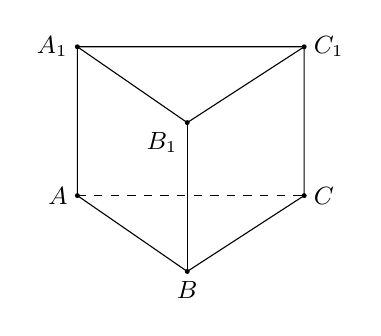
\begin{tikzpicture}[>=stealth, scale=0.9, font=\small]
  \coordinate (A)  at (0,1.45);
  \coordinate (C)  at (3.20,1.45);
  \coordinate (B)  at (1.55,0.38);
  \coordinate (A1) at (0,3.55);
  \coordinate (B1) at (1.55,2.48);
  \coordinate (C1) at (3.20,3.55);
  % 可见棱
  \draw (A1) -- (C1) -- (C) -- (B) -- (A) -- (A1);
  \draw (A1) -- (B1) -- (C1);
  \draw (B1) -- (B);
  % 不可见棱
  \draw[dashed] (A) -- (C);
  % 顶点
  \fill (A) circle (1pt) node[left] {$A$};
  \fill (B) circle (1pt) node[below] {$B$};
  \fill (C) circle (1pt) node[right] {$C$};
  \fill (A1) circle (1pt) node[left] {$A_1$};
  \fill (B1) circle (1pt) node[below left] {$B_1$};
  \fill (C1) circle (1pt) node[right] {$C_1$};
\end{tikzpicture}
\end{center}
\nopagebreak[4]
\Needspace{0.4\textheight}
\end{question}
\begin{question}
\gkti{26}\textbf{（本题满分 7 分）} 如图，某校有一块形如直角三角形 $ABC$ 的空地，其中 $\angle B$ 为直角，$AB$ 长 $40$ 米，$BC$ 长 $50$ 米，现欲在此空地上建造一间健身房，其占地形状为矩形，且 $B$ 为矩形的一个顶点，求该健身房的最大占地面积。
\nopagebreak[4]
\begin{center}% 2013 年春季上海卷第 26 题：直角三角形 ABC 与内接矩形 EBFP
% 图中 AB=4、BC=5 仅为示意比例；矩形 E-B-F-P 的顶点 P 在斜边 AC 上。
\begin{tikzpicture}[>=stealth, scale=1.0, font=\small]
  \coordinate (B) at (0,0);
  \coordinate (C) at (5.0,0);
  \coordinate (A) at (0,4.0);
  \coordinate (E) at (0,2.0);
  \coordinate (F) at (2.5,0);
  \coordinate (P) at (2.5,2.0);
  \draw (A) -- (B) -- (C) -- cycle;
  \draw (E) -- (B) -- (F) -- (P) -- cycle;
  % 直角标记
  \draw (0,0.32) -- (0.32,0.32) -- (0.32,0);
  % 顶点
  \fill (A) circle (1pt) node[above] {$A$};
  \fill (B) circle (1pt) node[below left] {$B$};
  \fill (C) circle (1pt) node[below right] {$C$};
  \fill (E) circle (1pt) node[left] {$E$};
  \fill (F) circle (1pt) node[below] {$F$};
  \fill (P) circle (1pt) node[right] {$P$};
\end{tikzpicture}
\end{center}
\nopagebreak[4]
\end{question}
\begin{question}
\gkti{27}\textbf{（本题满分 8 分）} 已知数列 $\{a_n\}$ 的前 $n$ 项和为 $S_n=-n^2+n$，数列 $\{b_n\}$ 满足 $b_n=2^{a_n}$，求 $\displaystyle\lim_{n\to\infty}(b_1+b_2+\cdots+b_n)$。

\end{question}
\begin{question}
\gkti{28}\textbf{（本题满分 13 分）} 本题共有 $2$ 个小题，第 $1$ 小题满分 $4$ 分，第 $2$ 小题满分 $9$ 分。

已知椭圆 $C$ 的两个焦点分别为 $F_1(-1,0)$、$F_2(1,0)$，短轴的两个端点分别为 $B_1$、$B_2$。

（1） 若 $\triangle F_1B_1B_2$ 为等边三角形，求椭圆 $C$ 的方程；

（2） 若椭圆 $C$ 的短轴长为 $2$，过点 $F_2$ 的直线 $l$ 与椭圆 $C$ 相交于 $P$、$Q$ 两点，且 $\overrightarrow{F_1P}\perp\overrightarrow{F_1Q}$，求直线 $l$ 的方程。

\end{question}
\begin{question}
\gkti{29}\textbf{（本题满分 12 分）} 本题共有 $2$ 个小题，第 $1$ 小题满分 $6$ 分，第 $2$ 小题满分 $6$ 分。

已知抛物线 $C:y^2=4x$ 的焦点为 $F$。

（1） 点 $A$、$P$ 满足 $\overrightarrow{AP}=-2\overrightarrow{FA}$。当点 $A$ 在抛物线 $C$ 上运动时，求动点 $P$ 的轨迹方程；

（2） 在 $x$ 轴上是否存在点 $Q$，使得点 $Q$ 关于直线 $y=2x$ 的对称点在抛物线 $C$ 上？如果存在，求所有满足条件的点 $Q$ 的坐标；如果不存在，请说明理由。

\Needspace{0.4\textheight}
\end{question}
\begin{question}
\gkti{30}\textbf{（本题满分 13 分）} 本题共有 $2$ 个小题，第一小题满分 $4$ 分，第二小题满分 $9$ 分。

在平面直角坐标系 $xOy$ 中，点 $A$ 在 $y$ 轴正半轴上，点 $P_n$ 在 $x$ 轴上，其横坐标为 $x_n$，且 $\{x_n\}$ 是首项为 $1$、公比为 $2$ 的等比数列，记 $\angle P_nAP_{n+1}=\theta_n$，$n\in\mathbf N^*$。
\nopagebreak[4]
\begin{center}% 2013 年春季上海卷第 30 题：y 轴正半轴上的点 A 与 x 轴上的点列 P1,P2,P3,P4
% 各射线自 A 引出；P4 之后以点列省略号表示继续。
\begin{tikzpicture}[>=stealth, scale=1.0, font=\small]
  \coordinate (O) at (0,0);
  \coordinate (A) at (0,3.4);
  \coordinate (P1) at (1.05,0);
  \coordinate (P2) at (1.80,0);
  \coordinate (P3) at (2.75,0);
  \coordinate (P4) at (4.40,0);
  \draw[->] (0,0) -- (7.10,0) node[below] {$x$};
  \draw[->] (0,0) -- (0,4.05) node[left] {$y$};
  \node[below left] at (0,0) {$O$};
  \foreach \p in {P1,P2,P3,P4}{
    \draw (A) -- (\p);
    \fill (\p) circle (1.3pt);
  }
  % 点列省略号
  \fill (5.55,0) circle (0.7pt);
  \fill (5.85,0) circle (0.7pt);
  \fill (6.15,0) circle (0.7pt);
  \fill (A) circle (1.3pt) node[left] {$A$};
  \node[below] at (P1) {$P_1$};
  \node[below] at (P2) {$P_2$};
  \node[below] at (P3) {$P_3$};
  \node[below] at (P4) {$P_4$};
\end{tikzpicture}
\end{center}
\nopagebreak[4]
（1） 若 $\theta_3=\arctan\dfrac13$，求点 $A$ 的坐标；

（2） 若点 $A$ 的坐标为 $(0,8\sqrt2)$，求 $\theta_n$ 的最大值及相应 $n$ 的值。

\end{question}
\begin{question}
\gkti{31}\textbf{（本题满分 18 分）} 本题共有 $3$ 个小题，第 $1$ 小题满分 $5$ 分，第 $2$ 小题满分 $7$ 分，第 $3$ 小题满分 $6$ 分。

已知真命题：“函数 $y=f(x)$ 的图像关于点 $P(a,b)$ 成中心对称图形”的充要条件为“函数 $y=f(x+a)-b$ 是奇函数”。

（1） 将函数 $g(x)=x^3-3x^2$ 的图像向左平移 $1$ 个单位，再向上平移 $2$ 个单位，求此时图像对应的函数解析式，并利用题设中的真命题求函数 $g(x)$ 图像对称中心的坐标；

（2） 求函数 $h(x)=\log_2\dfrac{2x}{4-x}$ 图像对称中心的坐标；

（3） 已知命题：“函数 $y=f(x)$ 的图像关于某直线成轴对称图像”的充要条件为“存在实数 $a$ 和 $b$，使得函数 $y=f(x+a)-b$ 是偶函数”。判断该命题的真假。如果是真命题，请给予证明；如果是假命题，请说明理由，并类比题设的真命题对它进行修改，使之成为真命题（不必证明）。

\end{question}